\section{Phases d'OCR}
Pour arriver à extraire le texte se trouvant sur un document, la technologie OCR le fait passer par une succession de plusieurs étapes.
    \subsection{Prétraitement}
    L’objectif de cette étape est d’améliorer la qualité de l’image et de faciliter son traitement pour de meilleurs résultats. Pour cela, on utilise quelques méthodes comme:
    \begin{itemize}
        \item[•]\textbf{La binarisation}: il s'agit de convertir une image en couleur qui est en trois dimensions en une image bidimensionnelle noir sur blanc. Pour cela, on passe par une étape intermédiaire
        appelée le \textit{grayscaling} qui convertit l'image en gris et en utilisant le seuillage sur l'image obtenue pour aboutir à une image en noir et blanc.
        \item[•]\textbf{Le redressement}: lors du processus de numérisation des documents, il peut y arriver
        quelques déformations sur le document numérisé obtenu. Ces déformations peuvent être des
        inclinaisons du texte. Cette étape permet de redresser l'image afin que les textes par exemple
        soient placées horizontalement.
        \item[•]\textbf{Le zonage}: il permet de selectionner la partie de l'image où l'on veut extraire les informations.
        \item[•]\textbf{Le suppression des bruits}: ici on enlève les éléments qui peuvent être considérés comme du bruit de l'image. Ceci peut être des lignes verticales, horizontales, obliques, des points en arrière plan.
        \item[•]\textbf{L'amincissement et la squelettisation }: il permet d'uniformiser la taille du texte dans l'image.   
    \end{itemize}
    \begin{figure}[H]
        \centering
        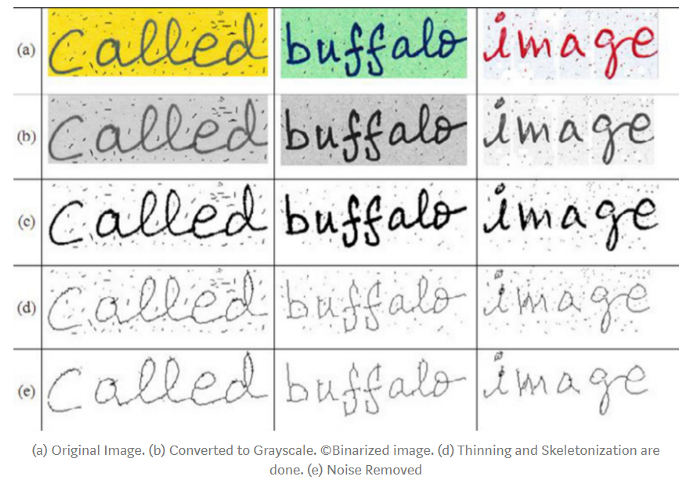
\includegraphics[scale=0.5]{preprocessing.png}
        \caption{Phases de prétraitement}
    \end{figure}
    \subsection{Segmentation}
    Le but de cette phase est d'isoler les lignes et les  caractères se trouvant sur l'image. Il existe donc trois types de segmentation:
        \begin{itemize}
            \item[•]\textbf{La segmentation des lignes} : l'objectif principal de ce type est de déterminer les coordonnées des lignes dans l'image, ce qui peut diviser l'image en lignes. L’idée est que, si nous projetons horizontalement l'image binaire, les lignes qui ont les pixels de texte ont des pics plus élevés, en raison du plus grand nombre de pixels de premier plan et les lignes qui ont l'espacement entre les lignes ont des pics plus faibles, en raison du plus grand nombre de pixels d'arrière-plan. 
            \item[•]\textbf{La segmentation des mots}: l'objectif principal de ce type est de déterminer où nous devons segmenter l'image pour séparer les mots. L’idée est la même que l'étape précédente, mais le seul changement est ici que nous projetons l'image verticalement parce que nous séparons les mots verticalement. Les colonnes qui ont les pixels de texte ont des pics plus élevés, en raison de plus de nombre de pixels de premier plan et les colonnes qui ont l'espace entre les mots contiennent des pics plus faibles, en raison de plus de nombre de pixels d'arrière-plan.
            \item[•]\textbf{La segmentation des caractères} : la tâche de la segmentation au niveau des caractères consiste à séparer les caractères uniques (comme les alphabets, les chiffres et autres symboles) des mots qui sont séparés de l'étape précédente.
        \end{itemize}
    Grosso modo, on a deux types de projections pour segmenter les images:
        \begin{itemize}
            \item[•]\textbf{La projection horizontale} : utilisée dans la segmentation au niveau des lignes.
            \item[•]\textbf{La projection verticale}: utilisée dans la segmentation au niveau des mots et des caractères.
        \end{itemize}
    \begin{figure}
        \centering
        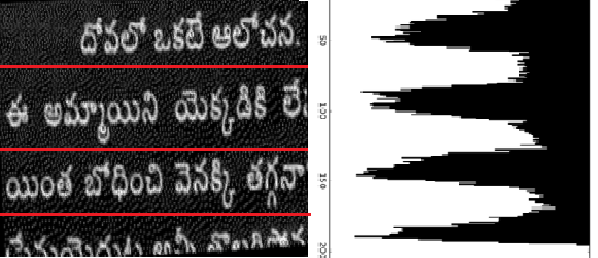
\includegraphics[scale=0.5]{segmentationLignes.png}
        \caption{Segmentation des lignes par projection horirontale}
    \end{figure}
    \begin{figure}
        \centering
        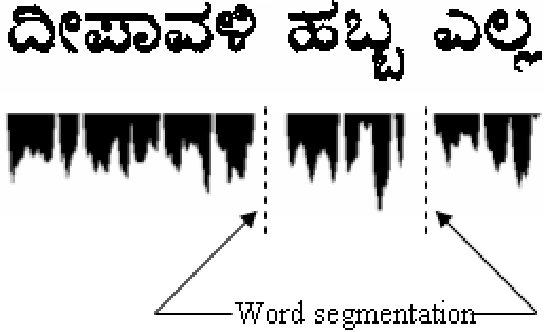
\includegraphics[scale=0.5]{segmentationMots.png}
        \caption{Segmentation des mots par projection verticale}
    \end{figure}
    \subsection{Reconnaissance de caractères}
    Le but est d'identifier numériquement le caractère qui est en image. Pour y parvenir, il existe des techniques de reconnaissance qui peuvent classées en trois grands groupes:
        \begin{enumerate}
            \item \textbf{La classification par caractéristiques (Features)}: une forme à reconnaître est représentée par un vecteur de valeurs numériques - appelées features en anglais - calculées à partir de cette forme. Le nombre de features est de l'ordre de 100 à 300. Si les features sont bien choisies, une classe de caractères (par exemple l'ensemble des A majuscules) sera représentée par un « nuage » contigu de points dans l'espace vectoriel des features. Le rôle du classificateur est de déterminer à quel nuage (donc à quelle classe de caractères) la forme à reconnaitre appartient le plus vraisemblablement. La classification fait généralement appel à divers types de réseaux de neurones artificiels entrainés sur de vastes bases de formes possibles.
            \item \textbf{Les méthodes métriques} : consistent à comparer directement la forme à reconnaître, au moyen d'algorithmes de distance, avec un ensemble de modèles appris. Ce type de méthode est peu utilisé et peu valorisé par les chercheurs, car souvent plus naïf et vraisemblablement moins efficace que les méthodes à base de features.
            \item \textbf{Les méthodes statistiques}: dans le domaine de la reconnaissance d'écriture manuscrite, il est fréquemment fait appel aux méthodes probabilistes comme les chaînes de Markov.\cite{wikiOCR}
        \end{enumerate}

    \subsection{Post-traitement}
    L'objectif de cette phase est de reduire les erreurs de reconnaissance. On utilise à cet effet des méthodes linguistiques et contextuelles pour identifier les mauvaises reconnaissances et proposer une éventuelle correction. 